% https://www.springer.com/gp/computer-science/lncs/conference-proceedings-guidelines
\documentclass[runningheads]{llncs}
%
\usepackage[left=2.5cm, right=2.5cm, top=2.5cm, bottom=2.5cm]{geometry}
\usepackage[T1]{fontenc}
% T1 fonts will be used to generate the final print and online PDFs,
% so please use T1 fonts in your manuscript whenever possible.
% Other font encondings may result in incorrect characters.
%
\pagestyle{plain}
\usepackage{graphicx}
\usepackage{float}
\usepackage{hyperref}
\usepackage{amsmath}
\usepackage{parselines}
\usepackage{listings}
% Used for displaying a sample figure. If possible, figure files should
% be included in EPS format.
%
% If you use the hyperref package, please uncomment the following two lines
% to display URLs in blue roman font according to Springer's eBook style:
%\usepackage{color}
%\renewcommand\UrlFont{\color{blue}\rmfamily}
%\urlstyle{rm}
%
\begin{document}
%
% todo: set this
\title{CRC - Incipient Cognition}


%
%\titlerunning{Abbreviated paper title}
% If the paper title is too long for the running head, you can set
% an abbreviated paper title here
%
\author{José Moniz\orcidID{110960} \and Miguel Albuquerque\orcidID{1105828} \and
Pedro Baptista\orcidID{96302}}

\institute{Instituto Superior Técnico, Av. Rovisco Pais 1, 1049-001 Lisboa, Portugal \\
\email{\{jose.f.moniz, miguel.albuquerque, pedro.maria.baptista\}@tecnico.ulisboa.pt}}


%
\maketitle              % typeset the header of the contribution
%

\keywords{Incipient Cognition \and Spatial Structure \and Prisoner's Dilemma \and
Cooperation \and Payoff}


\begin{abstract}
The evolution of cooperation in dynamic systems, particularly in distributed networks,
is a significant focus in evolutionary game theory. These systems model agent
interactions where decisions to cooperate or defect shape long-term network stability.
In this study, we replicate and confirm the results of Vukov et al. \cite{vukov},
demonstrating that incipient cognition—the ability of agents to adapt
strategies based on prior interactions—significantly enhances cooperation in spatial networks.
Through simulations with varying configurations, we observe that incipient cognition fosters
cooperation even under high temptation to defect. Our findings highlight the
robustness of cooperation when agents employ cognitive strategies, and how factors
like noise in strategy adoption do not prevent cooperative behavior.
These results reinforce the theoretical predictions and provide strong evidence
for applying these models to real-world scenarios.

\end{abstract}



\section{Introduction}

\subsection{Background}


\textbf{Prisoner's Dilemma} is one of the Metaphors for understanding the evolution of cooperation
in multiple fields like economics, evolutionary biology, computer science, etc \cite{mm2024}.
The rational goal is for an individual to maximize its own payoff however, facing a
dilemma: although mutual cooperation is better than mutual defection, individual rational
choice leads to mutual defection. Yet, cooperation surrounds us and is the most suited
strategy in some cases like in evolutionary biology. The takeaway is, assuming
an infinite population: the strategy whose fitness exceeds the average fitness
of the population will increase in frequency otherwise, the strategies that do not,
decline \cite{mm2024}. Furthermore, the choice of cooperation versus defection are
subject to changing probabilities, as different cost-to-payoff matrices lead to
different dilemmas of cooperation, i.e., temptation to defect.
This will also be observed from this study.

\textbf{Direct Reciprocity} is concerned with the positive action from Agent 1
to Agent 2, and Agent's 2 positive reciprocity, i.e., mutual cooperation.

\textbf{Incipient Cognition} is the capability to recall past actions and is
a pilar for direct reciprocity, as direct reciprocity
relies on the individual's experience and memory.

\textbf{Regular Lattices} are characterized by their regular structure and fixed
number of neighbors. These were used in this study, more precisely,
2D grid lattices, meaning k neighbors, where k=4. This regular topology is of relevance
for the conclusions gathered regarding spatial reciprocity.

\textbf{An Homogeneous Network} is a the kind of network produced by 2D
grid lattices. This means that all agents are equally connected, i.e.,
interaction and influence is distributed evenly, and this is also
another characteristic that promotes cooperating clusters that can shield themselves
from defectors.

\begin{figure}[htbp]
    \centering
    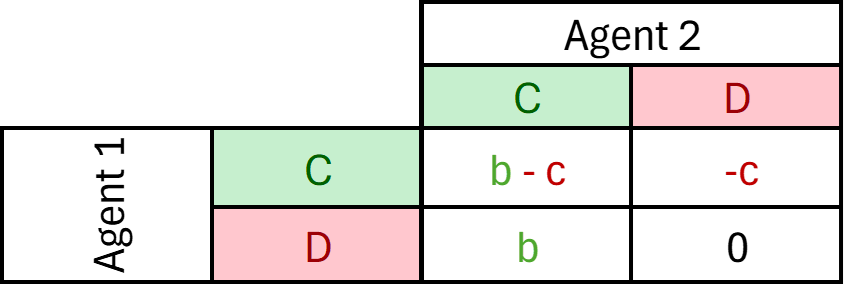
\includegraphics[width=0.4\textwidth]{payoffmatrix.png}
    \caption{Prisoner's Dilemma Payoff Matrix}
    \label{fig:coop_vs_b}
\end{figure}



\subsection{Motivation and Related Work}
The evolution of cooperation in dynamic systems is a central question in evolutionary
game theory, with implications for fields ranging from biology to social networks
and distributed control systems \cite{nowak2006}. Cooperation, although beneficial for the collective,
is often undermined by defection, where individual agents seek short-term gains at
the expense of collective well-being \cite{axelrod1981}. The Prisoner’s Dilemma (PD) offers a
fundamental framework for examining such interactions, presenting agents with a
choice between cooperation and defection, and its dynamics have been widely studied
to understand the conditions under which cooperation can emerge and persist \cite{nowak1992}.

Spatial structure has long been recognized as a crucial factor in promoting cooperation.
When agents are embedded in spatially structured networks, such as grids or lattices,
cooperative clusters can form and resist invasion by defectors. However, spatial
reciprocity alone is often insufficient to ensure long-term cooperation, especially
under high temptation to defect \cite{nowak1992,szabo2007}.


Recent studies, including the work by Vukov et al. \cite{vukov}, introduced the concept of incipient
cognition to address this limitation.
Incipient cognition allows agents to adapt their strategies based on previous
interactions, providing a more dynamic and flexible approach to decision-making.
By allowing agents to remember and react to past experiences, cognitive abilities
can significantly enhance cooperation, even in environments where defection might
otherwise dominate. Vukov et al. demonstrated that incorporating these cognitive
abilities into agents' decision-making processes led to robust cooperation,
even under conditions of high temptation to defect.

In this study, we replicate and extend the findings of Vukov et al. \cite{vukov},
confirming the impact of incipient cognition on the evolution of cooperation in
spatial networks and by implementing the studied paper, we further explore the
robustness of cooperation in heterogeneous networks where agents have incipient cognition
and dynamic systems.
Our results align with the theoretical predictions, demonstrating that agents
employing incipient cognition maintain high levels of cooperation, even under
significant temptation to defect.

\section{Methods/Model}

\subsection{Baseline: Previous Work}

The foundational work by Vukov et al. \cite{vukov} explored how incipient cognition, coupled with
spatial structure, promotes cooperation in a Prisoner’s Dilemma setting.
In this paper's model, agents occupied nodes on a network and interacted only with their
immediate neighbors. Each agent's decision to cooperate or defect was influenced
by prior interactions, allowing for adaptive strategies based on the last behavior.
Fitness, calculated as the accumulated payoff from repeated interactions,
determined strategy evolution. Agents adopted the strategies of more successful
neighbors probabilistically, with occasional mutations introducing a stochastic
mechanism into the process.

Their results highlighted the crucial role of spatial structure in facilitating cooperation.
Cooperative agents tended to cluster, protecting themselves from defection and
sustaining cooperation over time. Vukov et al. \cite{vukov} also found that the
temptation to
defect, represented by the parameter \( b \), played a pivotal role in determining
the sustainability of cooperation. Notably, their model already incorporated
cognition-based strategy adaptation, where agents adjust their behaviors based on
previous interactions, leading to the formation of robust cooperative clusters even
under conditions of temptation.


\subsection{Our Approach: Implementation and Simulation Setup}

To replicate and further examine the role of cognitive adaptation in promoting
cooperation, we implemented a model that builds upon the framework established
by Vukov et al. \cite{vukov}.

Each agent in our implementation, similarly to the referenced paper, was defined by
two evolving parameters:

\[
p: \text{Probability of cooperating after a cooperative interaction.}
\]

\[
q: \text{Probability of cooperating after a defecting interaction.}
\]


\begin{figure}[htbp]
    \centering
    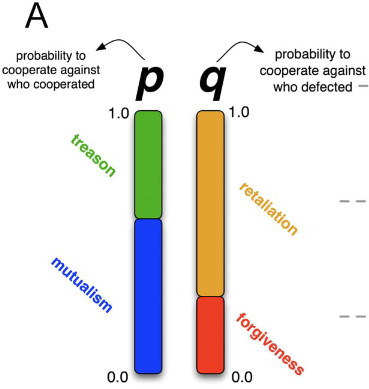
\includegraphics[width=0.4\textwidth]{modellingindividualcognition.png}
    \caption{Individual cognition model (in Results and Discussion of \cite{vukov})}
    \label{fig:coop_vs_b}
\end{figure}

These parameters were updated as agents interacted with their neighbors, allowing
for a dynamic adjustment of strategies based on the outcome of previous interactions.
The evolution happened in each simulation time step,
i.e., after each agent-to-agent play and was applied by picking two random
neighboring players (x and y). The adoption strategy happens with a probability
given by $W(x \leftarrow y) = \frac{1}{1 + e^{(P_x - P_y)/k}}$, where $P_x$ and $P_y$
are the fitness of agents x and y, and $K$ represents errors in decision making,
where the value used was 4, like in Vukov et al. \cite{vukov}.
Additionally, we also introduced stochastic noise whenever the agent x is
adopting the strategy of agent y, simulating small random fluctuations in the
values of \( p \) and \( q \).
This noise added an element of variability to the agents' decision-making,
reflecting more realistic cognitive decision-making processes compared to
purely deterministic models.


Simulations were conducted on a \( 30 \times 30 \) lattice, with each agent interacting
with its direct nearest neighbors (Von Neumann neighborhood). We systematically
varied the temptation to defect, denoted by \( b \) (b$=$\{1.0, 1.2, 1.4, 1.6, 1.8, 2.0\}), across multiple simulation
runs to assess the sensitivity of cooperation to this parameter. Each simulation
ran for 25,000 generations, with a transient period included to allow the system
to stabilize before data collection. The transient period used was $latticeSize^2$,
i.e., $50^2 = 2500$.

Our approach confirmed the results of Vukov et al. \cite{vukov}, demonstrating that
incipient cognition, when coupled with spatial structures, leads to robust
cooperation even under conditions of high temptation to defect.
The inclusion of incipient cognition in the model allowed us to further
explore (i) the nuances of how stochastic noise impacts results and (ii) the role
of adaptive decision-making to contribute to the persistence of cooperation.


\subsection{Additional Work}

In order to further extend the depth of the investigation, simulations were
implemented and conducted in order to see if the transient period initially
stated by Vukov et al. was sufficient for the values of p and q to become
somewhat stable, or if it was unsufficient, and if sufficient, if it was just
enough or too much.\\
These simulations were implemented the following way: a mean value of the
p and q values of all agents, in a single generation, is computed and added to an
array containing these said mean values from every generation. Then, as it only
was used one simulation (and not 10, as in the rest of this experiment, due
to the extremely high computational cost), this array is then used for the
final result that is shown in the next section.



\section{Results and Discussion}

\subsection{Comparison with Baseline Studies}
Previous research by Vukov et al. demonstrated that spatial structures within networks can sustain high levels of cooperation by forming clusters of cooperative agents. When the temptation to defect was low (\( b = 1.1 - 1.3 \)), these clusters provided a buffer against defectors, allowing cooperation levels to consistently exceed 80\%.

In our simulations, we were able to replicate these findings, confirming that cooperation remains robust under similar
conditions (\( b = 1.1 \)). By applying cognitive-based strategy
adaptation—where agents adjust their probabilities of cooperating based on
previous interactions—we observed similarly high levels of cooperation.
These results confirm the effectiveness of spatial structure and cognition in
promoting cooperation, even when stochastic elements such as noise are
introduced into the strategy evolution process.

\subsection{Insights from Cognitive Adaptation}
One of the key findings from our simulations is the importance of cognitive strategy adaptation in sustaining cooperation, even in the presence of stochastic noise. Similar to Vukov et al. model \cite{vukov}, our agents adopted strategies based on their past experiences with neighbors. The introduction of Gaussian noise allowed agents to slightly deviate from their neighbors' strategies, introducing variability that better reflects real-world decision-making processes.

\begin{figure}[H]
    \centering
    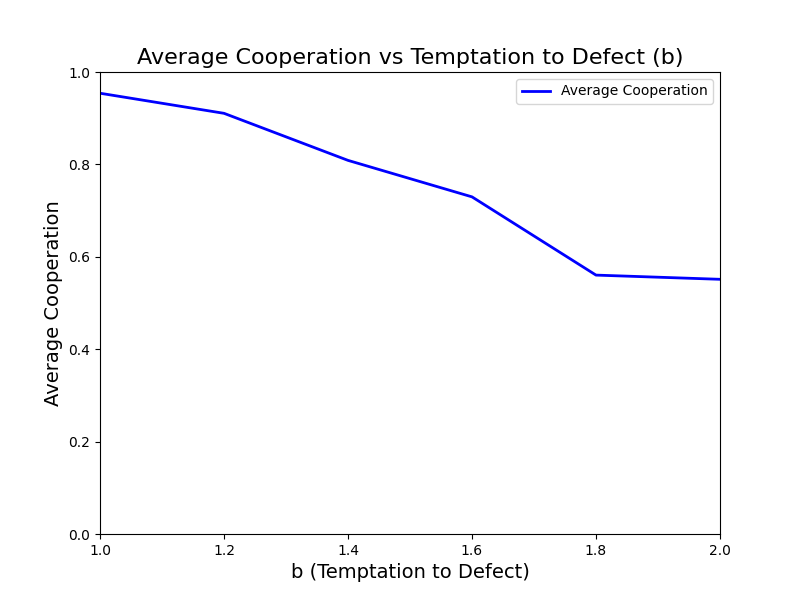
\includegraphics[width=0.7\textwidth]{cooperation_vs_b.png}
    \caption{Average Cooperation as a function of the temptation to defect (\( b \)). The plot shows how cooperation
    levels decrease as \( b \) increases, with significant drops when \( b > 1.2 \).}
    \label{fig:coop_vs_b}
\end{figure}

As expected, when the temptation parameter \( b \) ranged from 1.2 to 2.0, cooperation levels began to decline,
and defectors gradually increased their presence in the network.
While higher values of \( b \) naturally incentivize defection, the decline in
cooperation was gradual and followed the trends observed in Vukov et al. \cite{vukov}
results. This demonstrates that cognitive adaptation, even when paired
with stochastic noise, can sustain cooperation under moderate temptation but
faces challenges as \( b \) increases further.

\subsection{Additional Findings}
Our simulations also observed the significance of the transient period in the evolution
of cooperation. Early in the simulations, bursts of cooperation were observed
before the system stabilized at higher levels of cooperation.
This transient behavior indicates that agents need time to explore and
adapt their strategies before settling into more stable interaction patterns
, a phenomenon also noted by Vukov et al. \cite{vukov}.

Furthermore, the cognitive memory mechanisms in the model where agents
adjust their strategies based on
previous interactions introduced a level of complexity that goes beyond models with
fixed probabilities or static conditions, i.e., the opposite of dynamic decision making.
Cooperative bonds were maintained for longer periods in environments with lower
temptation values, but as \( b \) increased, the accumulated noise began to affect
these bonds. This finding emphasizes the trade-off between adaptability and stability,
where cognitive mechanisms allow for flexible decision-making but can also
introduce new challenges in maintaining long-term cooperation.

\begin{figure}[H]
    \centering
    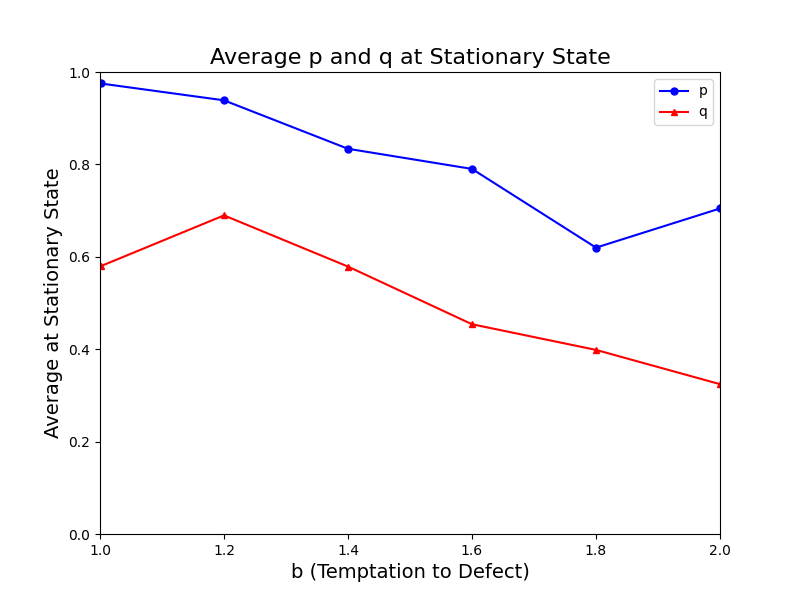
\includegraphics[width=0.7\textwidth]{p_q_vs_b.png}
    \caption{Average values of \( p \) (probability of cooperating after cooperation)
    and \( q \) (probability of cooperating after defection) as a function of \( b \).
    As \( b \) increases, both \( p \) and \( q \) decrease, reflecting a
    reduction in cooperation likelihood.}
    \label{fig:p_q_vs_b}
\end{figure}

In \ref{fig:p_q_vs_b} we can observe the general behavior, which is for values of
p and q to decrease as b increases, i.e., temptation to defect increases. At b=1.2
and b=2.0 we can see an increase on p and q, which is contrary to the expected behavior.
We can depict this result as an error in the simulation, and we believe that
by running more simulations, this contrary behavior would be rectified.



\subsection{Context and Broader Implications}
Our results, consistent with those of Vukov et al., reinforce the critical role
of cognitive mechanisms in sustaining cooperation within spatial networks.
Adding elements such as memory-based decision-making and stochastic noise
provides a more realistic simulation of real-world dynamics, where agents do
not always behave deterministically. Vukov et al. \cite{vukov} demonstrated that
spatial structure alone can promote cooperation, and our results confirm
that cognition-based strategy adaptation further enhances these effects, making
cooperation more resilient to variations in temptation to defect.

However, this realism comes with increased complexity. Cognitive adaptations introduce variability that may hinder cooperation under certain conditions, particularly when noise levels are high or temptation values exceed certain thresholds. These insights highlight the importance of balancing cognitive flexibility with strategy stability and underscore the need for further research into the interplay between noise and cognition in models of cooperation.

Our findings suggest that these models have significant potential for application in real-world systems, such as distributed networks and social platforms, where cooperation between agents is essential for system stability.
Future research should focus on exploring how adaptive noise levels and more
complex cognitive strategies can be applied to enhance cooperation in
increasingly dynamic environments.




\section{Conclusion}

\subsection{Limitations of Our Model and Methods}
While our model successfully replicated the results of Vukov et al. \cite{vukov}
and confirmed the role of cognitive mechanisms in promoting cooperation in
dynamic networks, several limitations remain. A key limitation is the
simplification of agent memory and decision-making processes. In our model,
agents base their strategies only on the most recent interaction, which may not
fully capture the cumulative effects of multiple interactions or long-term
relationships. This simplification may underestimate the potential for the formation
and stability of cooperative clusters over extended periods.

Furthermore, the use of Gaussian noise to introduce random mutations in strategy imitation, while valuable for adding variability, may overestimate the frequency and impact of random fluctuations in real-world systems. In practice, agents may not experience mutations as frequently or as randomly as modeled here, potentially leading to an overemphasis on instability in our results. Additionally, our model was limited to a lattice structure, which constrained our ability to explore more complex network topologies, such as small-world or scale-free networks. These structures could offer deeper insights into how different topological arrangements affect cooperation dynamics.

Another limitation resides in our simulations being confined to a specific range of temptation values (\( b \)) and fixed noise levels. While this range provided valuable insights, expanding the parameter space or introducing adaptive noise could provide a more comprehensive understanding of how these factors influence cooperation.

Lastly, the very high computational cost, in terms of temporal complexity, presents
a moderate issue. While we could not replicate the methodology of Vukov et al.,
which used a 100 by 100 lattice, as well as a larger number of simulations intended
to minimize the variation of the final results, our simulation still presented
a very approximate result of what we can expect from this kind of model in this
subject in particular.

\subsection{Future Work and Potential Applications}
Despite these limitations, our model opens several avenues for future research. Incorporating more sophisticated memory mechanisms into agent decision-making could offer a richer understanding of how long-term interactions shape cooperation. Future studies could explore how agents accumulate trust or mistrust over multiple rounds of interaction, influencing their probability of cooperating or defecting in subsequent games. Moving beyond the single-interaction memory used in our model, the introduction of "reputation," where agents base decisions on both direct interactions and the reputations of their neighbors, could provide deeper insights into the persistence of cooperation in more complex environments.

Moreover, extending our model to heterogeneous networks, where agents differ in both their initial strategies and their connectivity, would provide an important next step. Studies have shown that heterogeneous structures, such as those found in social and biological networks, can significantly affect the persistence of cooperation. Investigating how cognitive agents behave in such environments, especially when some agents hold more influence, could yield valuable insights into how network topology fosters cooperation.

Another promising area for future work is the study of adaptive noise levels. In our simulations, the noise level in strategy imitation was fixed throughout the generations, but in real-world systems, individuals may adjust their sensitivity to noise based on environmental factors or prior experiences. Allowing agents to modify their noise tolerance dynamically could reveal how agents balance exploration (trying new strategies) and exploitation (maintaining successful strategies) in evolving networks.

Finally, practical applications of this model could extend to distributed systems and social networks, where cooperation between individuals or agents is critical for maintaining system stability. Understanding how cognitive mechanisms influence cooperation can help inform the design of distributed decision-making algorithms and provide insights into encouraging cooperation in online platforms, organizations, and decentralized systems. By further exploring the interactions between cognition and network topology, future research can offer more robust strategies for fostering cooperation in a variety of real-world settings.

% ---- Bibliography ----
%
% BibTeX users should specify bibliography style 'splncs04'.
% References will then be sorted and formatted in the correct style.
%
% \bibliographystyle{splncs04}
% \bibliography{mybibliography}
%
\begin{thebibliography}{8}
\bibitem{mm2024}
Francisco, A, et al.: IST - Ciência de Redes Complexas - Class slides
Lisbon (2024)


\bibitem{vukov}
Vukov, J., Szabó, G., Szolnoki, A.: Cooperation in the noisy case: Prisoner's dilemma game on two types of regular random graphs. Physical Review E, 72(6), 067107 (2005)

\bibitem{nowak1992}
Nowak, M. A., May, R. M.: Evolutionary games and spatial chaos. Nature, 359(6398), 826-829 (1992)

\bibitem{nowak2006}
Nowak, M. A.: Five Rules for the Evolution of Cooperation. Science, 314(5805), 1560-1563 (2006)

\bibitem{szabo2007}
Szabó, G., Fáth, G.: Evolutionary games on graphs. Physics Reports, 446(4-6), 97-216 (2007)

\bibitem{axelrod1981}
Axelrod, R., Hamilton, W. D.: The evolution of cooperation. Science, 211(4489), 1390-1396 (1981)

\bibitem{szolnoki2013}
Szolnoki, A., Perc, M., Szabó, G.: Evolutionary dynamics of cooperation in neutral populations. Physical Review E, 87(5), 051101 (2013)

\bibitem{tanimoto2015}
Tanimoto, J.: Evolutionary Games with Sociophysics: Analysis of Traffic Flow and Epidemics. Springer (2015)

\end{thebibliography}

\end{document}
